%! Author = Antonio Lobo
%! Date = 30/10/2024

\section{Reduction Methods}
In this section, we briefly describe reduction techniques employed for instance-based learning. We use a simple 2D dataset for illustrative purposes.

\subsection{GCNN}


\subsection{EENTH}
This subsection outlines the Elimination Editing with Nearest-neighbor Threshold (EENTH) method \cite{vazquez2005}. This approach uses a modified $k$-NN rule, integrating probability-based decisions for instance elimination. The main steps are outlined below.

\begin{enumerate}
    \item \textbf{Probability-based Classification}: For each instance $ x $, calculate the probability $ p_i(x) $ of $ x $ belonging to each class $ i $ based on its $k$-nearest neighbors. Probabilities are weighted inversely by the distance to each neighbor and normalized:


	\begin{center}
	\begin{align}
		p_i^j &= \frac{|\{x_k \in NN_k(x) : y_k=j \}|}{k} \\
		P_i(x) &= \sum_{j=1}^{k} p_i^j \frac{1}{1 + d(x, x^j)} \\
		p_i(x) &= \frac{P_i(x)}{\sum_{j=1}^{M} P_j(x)}
	\end{align}
	\end{center}

    
    \item \textbf{Thresholding}: Define a threshold $ \mu $ to refine classification, we will denote as $p(x)$ the highest probability. Instances near decision boundaries, where $ p(x) < \mu $, are identified as candidates for removal.
    
    \item \textbf{Elimination}: If an instance $ x $ does not match the class with the highest probability, or if its highest class probability falls below $ \mu $, it is removed from the dataset, resulting in an edited set $ S \subseteq X $.
\end{enumerate}

The EENTH method thus provides a balance between retaining instances with high classification confidence and discarding uncertain instances near decision boundaries.

\subsection{DROP3}
In this subsection, we describe the basic concepts of the third method in the Decremental Reduction Optimization Procedure (DROP) family, as presented in Section 3 of Wilson et al. \cite{wilson2000reduction}. Although we will not delve into every detail, we describe the main ideas of the algorithm and illustrate them on $D_1$. See \textbf{Figure} \ref{fig:2dDataset}.

\begin{enumerate}
	\item \textbf{Remove noise}: The first step is to remove noisy instances using Edited Nearest Neighbor (EEN) \cite{wilson1972asymptotic}, where any instance misclassified by its $ k $-nearest neighbors is removed. The outcome of applying this technique is shown in \textbf{Figure} \ref{fig:2dEEN}, where noise has been removed. We denote the reduced dataset as $ T \subseteq D_1 $.
	\begin{figure}[ht]
		\centering
		\begin{minipage}{0.45\textwidth}
			\centering
			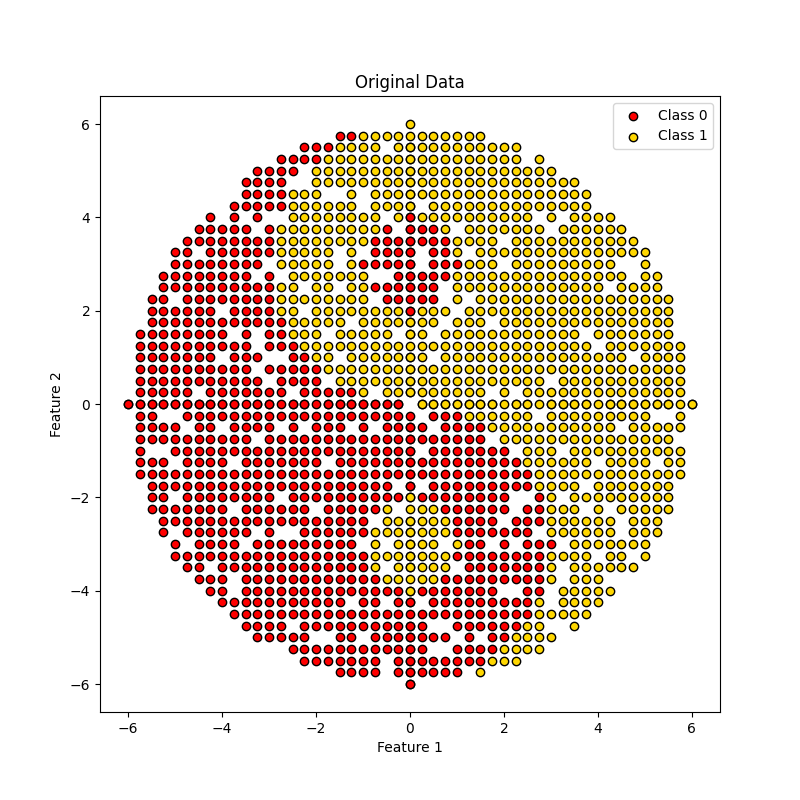
\includegraphics[width=\textwidth]{figures/2dDataset} % Adjust path and file name
			\caption{Original Dataset}
			\label{fig:2dDataset}
		\end{minipage}\hfill
		\begin{minipage}{0.45\textwidth}
			\centering
			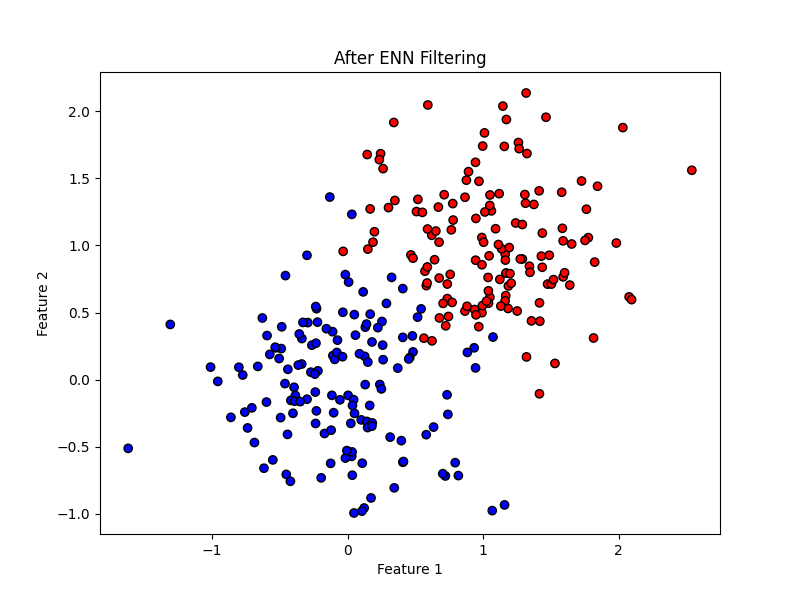
\includegraphics[width=\textwidth]{figures/2dEEN} % Adjust path and file name
			\caption{Effect of EEN}
			\label{fig:2dEEN}
		\end{minipage}
	\end{figure}
	
	\item \textbf{Sort points}: The next step is to prioritize removing points that are farthest from the decision boundary. For each point $ x_i \in S $ with class $ y_i $, we compute the distance to the nearest point with a different class, denoted as $ x_j \in D $ such that $ y_j \neq y_i $ and $ \nexists x_k : |x_k - x_i| < |x_j - x_i| \land y_i \neq y_k $.
	
	\item \textbf{Delete points}: Let $ S = T $. Starting with the points farthest from the boundary, we check if any associated points (points that have $ x_i $ as a neighbor) $ a_j $ receive more votes for their correct class with $ x_i $ as a neighbor (denoted as $ \text{with} $) or if they would be classified correctly if $ x_i $ were removed (denoted as $ \text{without} $). If $ \text{without} > \text{with} $, we remove $ x_j $ from $ S $, resulting in $ S' = S \setminus \{x_j\} $.
	
	\item \textbf{Selecting neighbors}: A key distinction between DROP1 and DROP2 is that DROP1 removes points that are removed from the dataset from the list of associates while DROP2 doesn't.
	
	\begin{figure}[ht]
		\centering
		\begin{minipage}{0.45\textwidth}
			\centering
			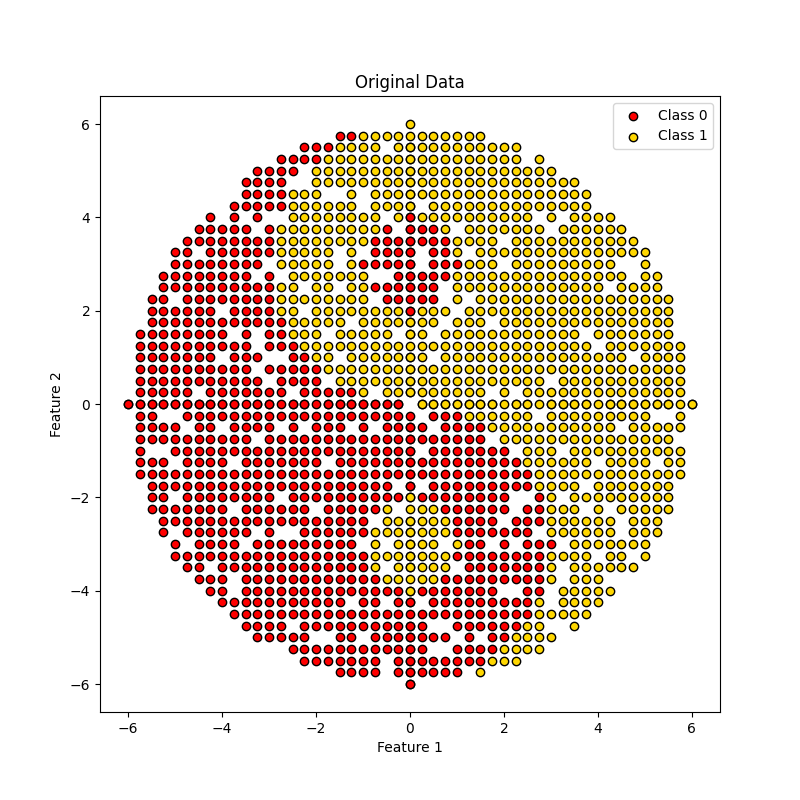
\includegraphics[width=\textwidth]{figures/2dDataset} % Adjust path and file name
			\caption{Original Dataset}
			\label{fig:2dDataset2}
		\end{minipage}\hfill
		\begin{minipage}{0.45\textwidth}
			\centering
			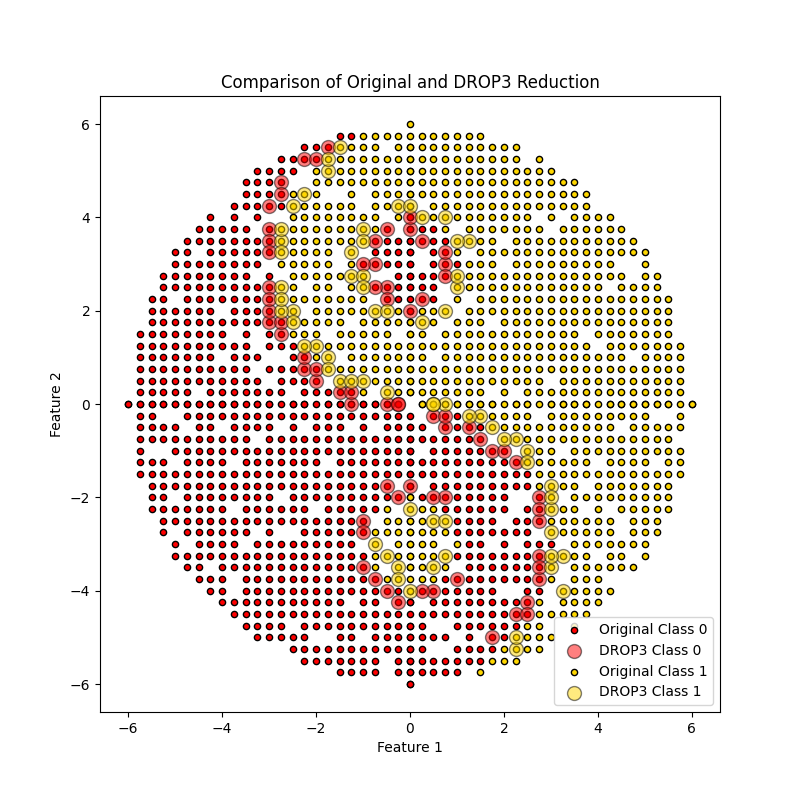
\includegraphics[width=\textwidth]{figures/DROP3} % Adjust path and file name
			\caption{Effect of DROP3}
			\label{fig:DROp3Total}
		\end{minipage}
	\end{figure}
	
\end{enumerate}
